\chapter{接口缺陷检测工具集与应用}
\label{cha:tools}
在代码质量保障中,规约描述语言能够有效的描述接口使用的约束体检、
高效的检测算法能够对大规模程序进行缺陷检测。
然而,这些已有成果离不开面向实际应用场景的工具集的支持。
直观地说,工具决定了语言描述、缺陷检测等成果在实际中的应用效果。
本文将第\ref{cha:impsec}章和\ref{cha:imchecker}章的研究成果应用于实际项目中,
并将结果总结在本章中。
具体来说,本章包含两部分内容:C程序接口缺陷数据集APIMU4C和
可视化支持的C程序接口缺陷检测工具集Tsmart-IMChecker。
APIMU4C包含对开源项目调研中找到的接口误用缺陷实例,
以及针对C程序的接口缺陷测试集。
Tsmart-IMChecker工具集包含三个子工具,
以帮助使用者方便高效地撰写IMSpec规约、执行分析引擎、基于差异性对比的分析检测结果。
同时,本章将Tsmart-IMChecker工具集应用于实际开源项目中,并对应用结果进行总结。
从全文的研究体系上看,
本章的工作旨在将接口描述语言IMSpec和规模化检测方法IMChecker应用于实际项目中,
体现前两章研究成果的实用性。

\section{引言}
过去的十几年内,研究人员与开发人员针对于C程序接口缺陷检测的工具设计和实现方面投入大量的时间和努力,
取得较好的研究成果。
例如,微软公司著名的接口缺陷检测项目SLAM,
被广泛使用的开源静态分析工具Cppcheck和Clang Static Analyzer等等。
特别地,为了给使用者提供更好的用户体验,这些工具都提供了良好的工具接口。
或通过命令行的方式直接调用工具进行检测,或者提供可视化支撑的GUI工具。
然而,针对于当下的开发环境和程序特点,以上方法存在若干不足。
为了弥补现有工作的不足,本文在第\ref{cha:impsec}章和\ref{cha:imchecker}章分别提出了基于缺陷模式的接口使用约束的领域特定语言IMSpec,
以及基于规约描述的规模化接口缺陷检测方法IMChecker。
本章将这两部分研究内容进行整理和封装,应用于实际开源项目中,并对应用结果进行总结。

首先,为了帮助研究人员和开发者更好的理解接口误用缺陷,
本章将缺陷调研以及算法评估中的原始数据集合进行整理和封装,
形成C程序接口缺陷数据集APIMU4C。
APIMU4C包含三个模块,即:
(1)面向Git版本控制库的修改记录挖掘工具Gitgrabber,
(2)开源项目接口缺陷案例库,
(3)基于公开数据集合以及实际项目的接口缺陷测试数据集。
APIMU4C包含本文中所有的原始数据集,
同时研究人员和开发者可以利用Gitgrabbger对其他领域的缺陷修复进行挖掘和提取。
此外,接口缺陷测试数据集能够帮助研究人员和开发者对现有工具进行评估,
以设计更具针对性的检测算法和选择适用的工具进行特定种类的缺陷检测。


为了提高工具的实用性,减轻使用者的负担,现有工具都提供良好的用户接口。
每个工具都有自己的特点,所针对的对象亦不同。
针对IMSpec语言和IMChecker检测方法,本文开发了相关的图形化支撑工具集Tsmart-IMChecker,
以提供更好的用户体验。
本工具集共包含三个主要模块,即:
(1)图形化规约撰写工具IMSpec-writer,通过点击、选择和填入必要语义信息的的方式,辅助开发者撰写规约;
(2)静态分析引擎IMChecker,通过对IMChecker方法的实现和封装,帮助开发者通过命令行的方式,直接调用分析引擎并生成对应的缺陷分析报告;
(3)图形化结果展示工具IMDisplayer,通过差异性结果展示的方式,帮助使用者快速、准确的定位缺陷。
本章将Tsmart-IMChecker应用于实际开源项目中,以检测工具的使用性。
工具集在Linux内核、OpenSSL和Ubuntu的应用软件的最新稳定版本中,
共发现75个实际缺陷。
作者将缺陷报告提交给相应开发者确认。
其中,62个已经被开发者确认,32个已经在主分支中修复。
本章中对实际应用中的困难和发现进行总结,以帮助研究人员和开发者设计更好的检测工具。



本章其余部分组织结构如下:
\ref{sec:4.2}节对APIMU4C数据集进行介绍;
\ref{sec:4.3}节介绍Tsmart-IMChecker工具总体架构和各子工具;
\ref{sec:4.4}节给出工具集在开源项目上的应用结果;
最后在\ref{sec:4.5}节总结本章工作。

\section{C程序接口误用数据集}
\label{sec:4.2}
近年来,软件缺陷获得了研究人员的广泛关注。
特别地,为了有效的比较缺陷检测工具的性能,
研究人员整理了针对不同领域和不同目的的数据。
例如,BugBench~\cite{05-bugbench}是针对C程序的缺陷评估集合,
共包含17个开源项目中的缺陷实例,
其中13个与内存、并发和语义相关。
Defects4J~\cite{14-issta-defects4j}是面向Java程序的缺陷集合,
共包含来自5个开源项目的357个缺陷实例。
在2016年,Amann等整理了MUBENCH~\cite{16-msr-mubench}数据集。
该数据集包含89个Java语言实际项目中的接口误用缺陷。
为了能够帮助研究人员和开发者更深入的理解接口误用缺陷,
本章整理了C程序接口误用数据集APIMU4C。
该数据集包含三个部分,面向Git版本控制库的修改记录挖掘工具Gitgrabber、
开源项目接口缺陷案例库、
以及基于公开数据集合以及实际项目的接口缺陷测试数据集。
本节将对每一个部分进行详细介绍,

\paragraph{Gitgrabber}
对于实际缺陷的分析有利于对缺陷本质的理解。
所以,无论是规约描述语言还是检测算法的设计,获得实际缺陷实例是重要基础。
随着软件复杂度增加和软件规模提升,现代软件难以独立完成。
同时随着网络的发展,越来越多的开发团队远程办公。
在众多的代码维护方式中,Git版本控制软件是最为广泛使用和最受欢迎的方式。
如图~\ref{fig:2-3-description}所示,开发者在使用Git版本控制软件时,
对于每一次修改记录,都会提供修改的描述报告。
Git会自动计算修改记录中代码的差异,生成差异报告。
因此,本文作者设计了Gitgrabber,面向Git版本控制软件的修改记录挖掘工具。
该工具基于Python语言设计,通过自然语言处理的方式对修改记录挖掘。
Gitgrabber需要用户提供配置文件,以提供挖掘的项目分支、关键词、
时间区间、个数、文件行数。
同时,Gitgrabber提供了多层挖掘服务,即在第一层挖掘结果的内容中,进行二次检索。
例如,通过缺陷修复的关键词进行缺陷修复相关修改记录挖掘。
再基于某种特定类型的关键词,挖掘特定领域的缺陷修复。
Gitgrabber使用方便,只需要提供基于结构化的描述的配置文件,并通过如下命令执行,
\begin{lstlisting}[language={bash},
basicstyle=\linespread{0.8}\listingsfont,
numbers=none,
xleftmargin=.3\textwidth]
(*@\textcolor{blue}{python}@*) main.py --config config.yml
\end{lstlisting}
挖掘的结果包括:修改记录报告、差异性报告、修改前文件和修改后的文件。
本文中缺陷模式调研的缺陷实例均来自于Gitgrabber的结果。

\paragraph{接口缺陷案例库}
理解缺陷模式是设计缺陷检测工具的重要基础。
所以,对实际项目中的缺陷进行分析,有利于研究人员和开发者更深入的理解缺陷的本质。
因此,本文作者将第~\ref{cha:impsec}章第~\ref{sec:2.3}节中分析的接口缺陷实例进行总结,
形成接口缺陷案例库。
目前该案例库共包含来自6个项目的830个实际接口误用缺陷实例,
其中Linux内核283个、OpenSSL127个、FFmpeg126个、Curl134个、FreeRDP119个以及Httpd41个。
作者对830个缺陷进行深入分析,以确保这些实例与接口误用相关。
同时,针对于每一个缺陷实例,我们收录了缺陷修复报告、差异性报告、修改前错误版本源文件以及
修改后正确版本源文件。
研究人员和开发者可以对这些案例进行研究,以设计更具有针对性的缺陷描述方法和检测方法。

\paragraph{接口缺陷测试集}
标准化的缺陷测试集合能有有效评估缺陷检测工具。
然而,目标并没有针对C程序接口误用缺陷的公开测试集合。
因此,作者基于公开数据集以及实际项目中的缺陷,构造了C程序接口缺陷数据集。
该数据集构成如表~\ref{tab:4-2-dataset}所示。
其中2172个为人工构造的单文件测试用例。
这些测试用例来源于广泛使用的公开测试集Juliet Test Suite和ITC~\cite{itc}。
每个测试用例在100-200行之间,涵盖不同的C语言的语法结构。
可以用来对检测工具的的语言支持度和检测策略进行分析。
测试集的另一部分为实际项目缺陷。
这些缺陷来源于缺陷调研的结果,并注入到项目的最新版本中。
可以用来评估检测工具在实际项目上的分析能力和效果。
这2272个缺陷集合包含了缺陷调研中常见的三种缺陷模式。
C程序接口缺陷数据集一方面能够帮助研究人员设计更具有针对性的检测算法。
另一方面,可以对现有工具进行评估,帮助研究人员分析现有工具不足。
同时使用者可以通过检测结果对工具的能力进行评估,以选择更使用的工具。

\begin{table}[t]
	\centering
	\begin{minipage}[t]{0.6\linewidth} % 如果想在表格中使用脚注,minipage是个不错的办法
		\caption{C程序接口误用缺陷测试集组成}
		\label{tab:4-2-dataset}
			\begin{tabular}{cccc}
			\hline
			缺陷位置 & 数目& 类型& 代码规模\\
			\hline
			单文件 & 2172 & 人工构造 & 100-200\\
			OpenSSL & 50 & 实际缺陷注入 & 454k\\
			Curl & 30 & 实际缺陷注入 & 113k\\
			Httpd & 20 & 实际缺陷注入 & 203k\\
			总计 & 2272 & \multicolumn{2}{c}{包含所有调研中出现的缺陷类型} \\
			\hline
		\end{tabular}
	\end{minipage}
\end{table}
\section{工具集组成}
\label{sec:4.3}
软件可信保障工具集Tsmart (Trustworthy Software System Modelling And Verification Toolkit),是清华大学软件学院软件系统与工程研究所研发的软件系统建模验证工具集。
Tsmart~\cite{tsmart}工具集在2019年1月发布第三版,是具有完全自主知识产权,面向软件代码安全可靠性的多维度保障体系。
Tsmart具有代码合规性分析、缺陷静态检测、缺陷自动修复、并发性属性分析等功能。
工具集可用于自动化地检测软件系统中难以发现、调试的重要缺陷,并给出相应的修复建议,从而提高软件系统的可靠性,以及软件开发测试效率,减小因为软件缺陷导致的损失。
Tsmart-IMChecker工具集是Tsmart的重要组成部分,面向C程序接口使用缺陷设计。
本节将对Tsmart-IMChecker的总体架构、模块组成进行介绍。

\subsection{总体架构}
Tsmart-IMChecker是基于可视化支持的C程序接口缺陷检测工具集。
如图~\ref{fig:4-3-overview}中所示,
工具集包含三个主要模块:
\begin{enumerate}
	\item IMSpec规约撰写工具:IMSpec语言提供了一套轻量级、类标记语言的语法结构,
	然而,手动撰写规约是一件耗时、容易出错的工作。因此本文设计了可视化支撑的IMSpec规约撰写工具,
	帮助用户描述接口使用约束。
	\item IMChecker分析引擎:本文将规模化检测方法实现于IMChecker分析引擎中,
	并提供基于命令行的使用接口。用户可以直接调用该接口进行缺陷检测,
	也可以将分析引擎嵌入到实际开发环境中,作为第三方插件使用。
	\item IMDisplayer结果展示工具。Tsmart工具集提供了基于网页版的可视化结果展示工具。
	为了帮助实际用户更好的理解接口使用缺陷发生原因,本文实现了基于差异性的结果展示工具。
	通过在同一个项目中,正确使用实例与缺陷实例的对比,突出接口误用的缺陷原因。
\end{enumerate}

\begin{figure}[t]
	\centering
	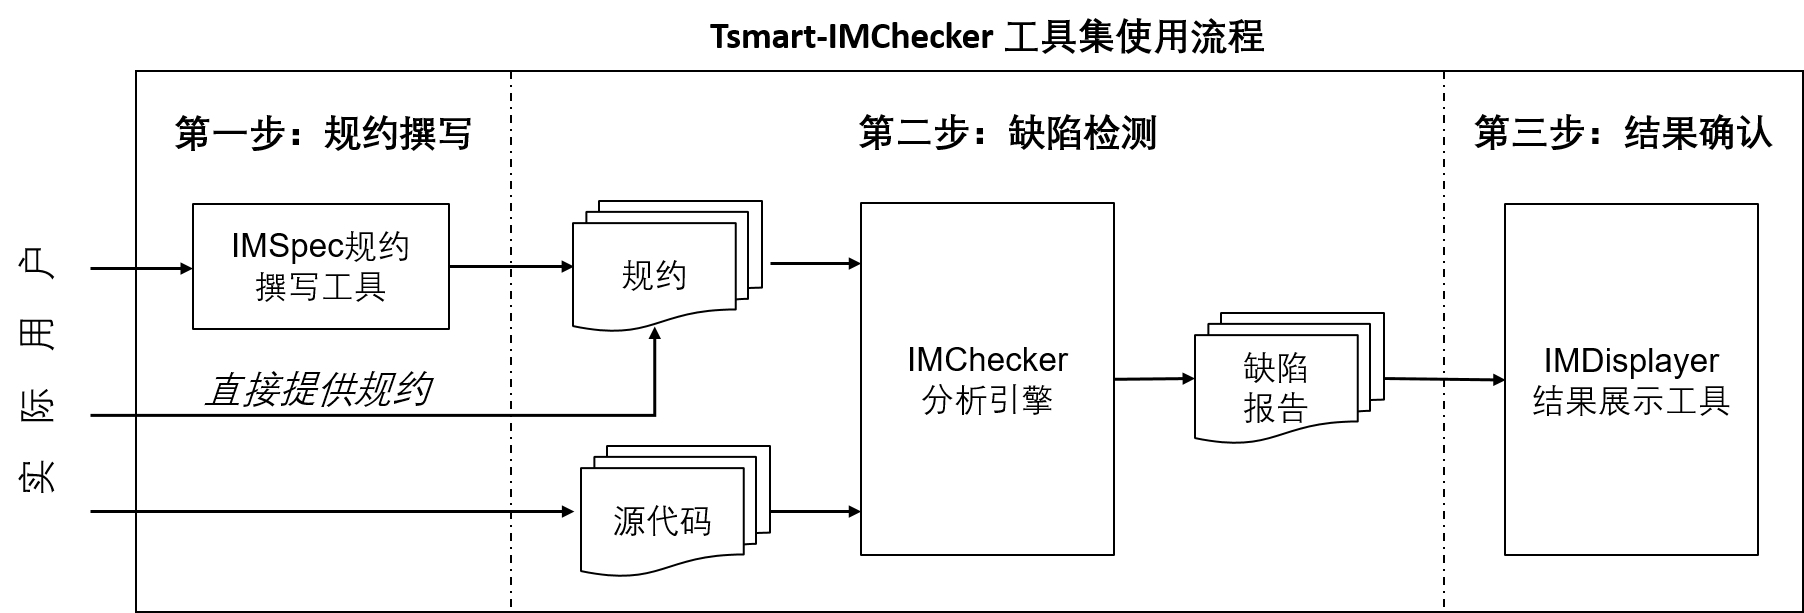
\includegraphics[width=0.85\linewidth]{figures/cp4-overview.png}
	\caption{
		Tsmart-IMChecker工具集使用流程。
	}
	\label{fig:4-3-overview}
\end{figure}

用户使用Tsmart-IMChecker工具进行接口缺陷检测需要三个步骤,即
(1)撰写规约,(2)缺陷检测,(3)结果确认。
首先,开发者通过IMSpec规约撰写工具,对目标接口的使用约束进行描述。
如果开发者理解IMSpec的语法结构,也可以通过直接撰写文本格式的规约描述。
在第二步,开发者通过调用缺陷检测引擎,基于提供的规约描述对源代码进行分析。
最后开发者可以直接通过生成的报告进行缺陷检测结果的核对,
也可以通过可视化的IMDisplayer工具对检测结果进行确认。
本节将在剩下的内容中,对每个模块进行详细介绍。



\subsection{规约撰写模块}
接口使用约束作为接口规约的一部分,已经被证明能能够有效的应用于软件工程领域的不同任务中。
特别地,这些规约能够帮助开发者理解如何正确使用API,
以及帮助测试人员对接口误用缺陷进行检测。
然而人工撰写这些约束条件需要大量的时间与经历,
同时容易在撰写中产生语法错误。
为了使用者减轻撰写IMSpec约束的负担、提高撰写规约语法的准确性,
本文设计并实现了图形化支撑的IMSpec规约撰写工具。

如图~\ref{fig:4-3-IMSpec-writer}中所示,IMSpec规约撰写工具包含三个部分:
\begin{itemize}
	\item {\kaishu 规约列表}
	界面的最左侧是规约列表,用于展示使用者已经完成的IMSpec接口约束实例。
	用户可以在列表中直观地了解已经完成的约束描述。
	目前IMSpec撰写工具将一个复杂规约会分解成多个子约束进行检测,以提高检测精度。
	因此,显示结果为分解后的约束条件。
	\item {\kaishu 编辑区} 
	界面的右侧为规约编辑区,用于对IMSpec规约进行编辑。
	编辑区包括三大主要区域:目标对象区域、前置条件编写和后置条件编写区域。
	用户在确定目标接口的名称和参数定以后,可以在下列的Ref区域选择性的填写与目标API相关的因果调用关系函数。
	例如:目标接口时\texttt{fopen()}函数,那么用户可以在Ref区域通过填写\texttt{fclose()}函数的定义强化因果调用关系。
	后续中,用户可以根据具体的接口使用约束,对前置条件和后置条件进行编辑。
	特别地,IMSpec规约撰写工具在IMSpec语法基础之上,
	在界面显示中进行了细微的调整,以提供更直观、准确的功能。
	在规约撰写中,用户可以使用宏定义以保持程序语义一致性。
	在缺陷检测阶段提供宏定义的头文件即可。
	\item {\kaishu 文件操作区} 
	界面的左下角是文件操作区域,包括加载宏定义文件、加载文件和导出三个功能。
	
\end{itemize}

用户通过命令行,执行imspec\_writer.py运行该工具:
\begin{lstlisting}[language={bash},
basicstyle=\linespread{0.8}\listingsfont,
numbers=none,
xleftmargin=.3\textwidth]
(*@\textcolor{blue}{Ubuntu@~:Python3}@*) imspec_writer.py
\end{lstlisting}
其运行结果被保存在用户选择的目录中的*.yaml文件中,
例如图~\ref{fig:2-4-example-imspec}中IMSpec实例。
此外,为了帮助使用者维持项目特定的语义及特殊定义,
IMSpec规约撰写工具提供了define.h文件共使用者定义宏参数。
例如针对于图~\ref{fig:2-4-example-imspec}中IMSpec实例,
用户可以在define.h中,定义如下宏:
\begin{lstlisting}[language={C},
basicstyle=\linespread{0.8}\listingsfont,
numbers=none,
xleftmargin=.3\textwidth]
#define SUCCESS 1
#define FILEERR -1
#define IOERR -2
\end{lstlisting}
则在后续的解析IMSpec语言时,解析会进行宏定义的展开,以和程序中的语义保持一致。

\begin{figure}[t]
	\centering
	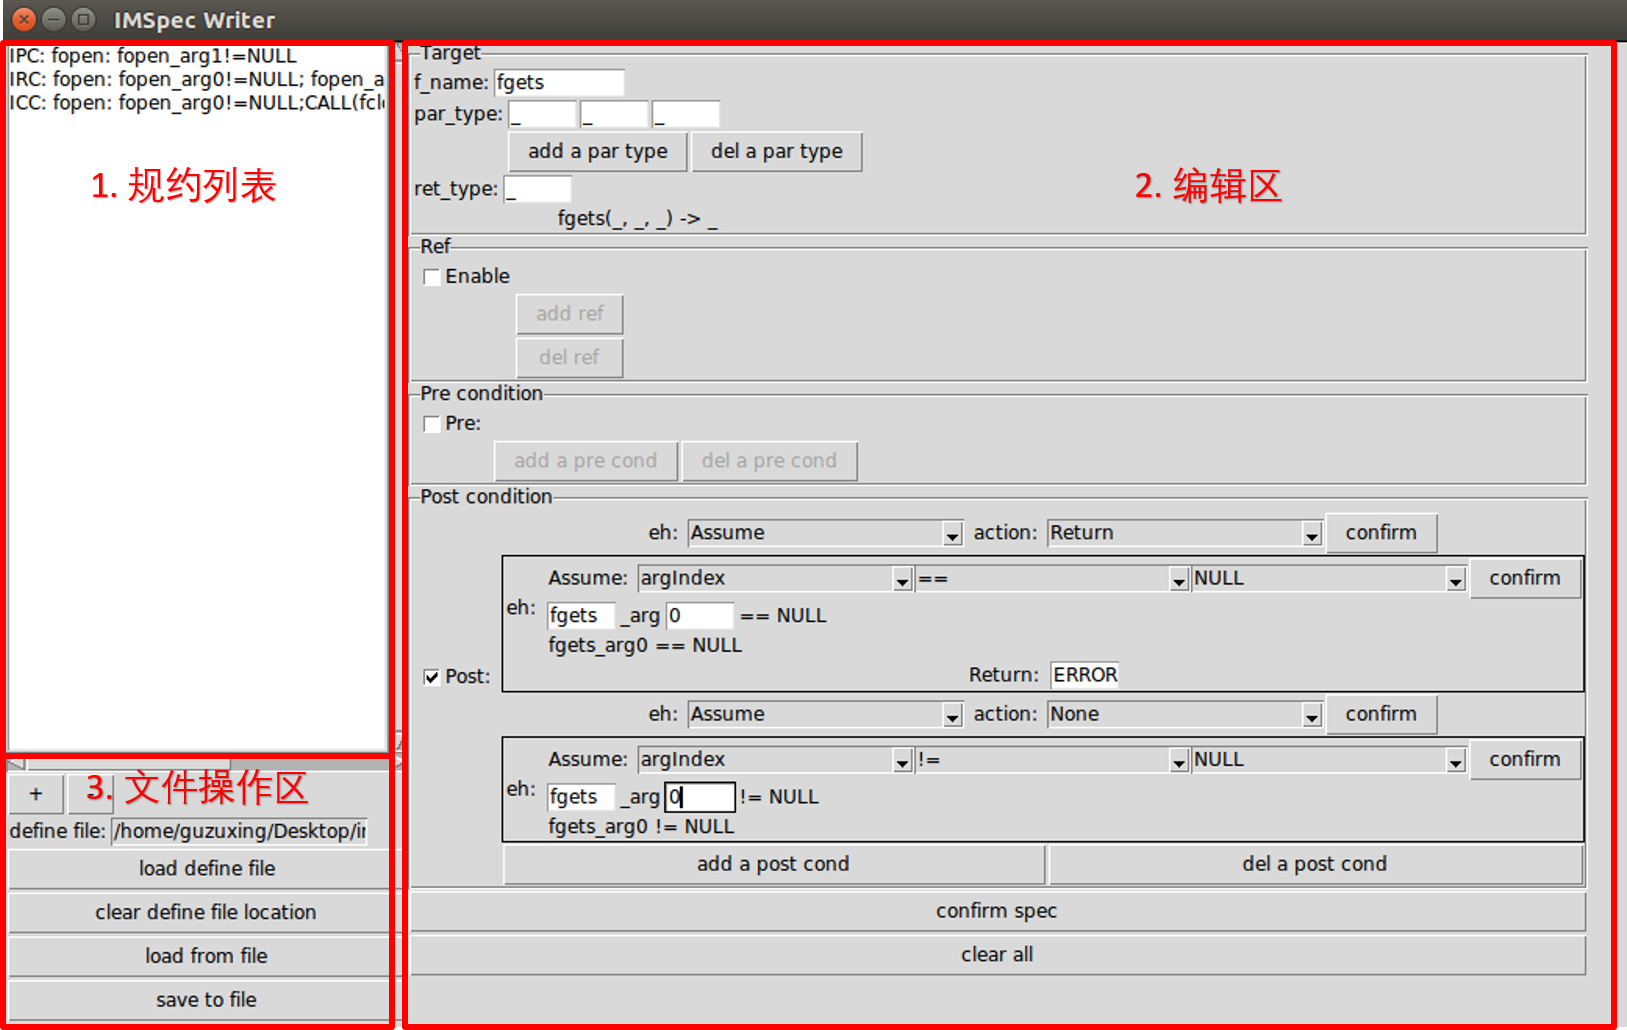
\includegraphics[width=0.85\linewidth]{figures/cp4-IMSpec-writer.png}
	\caption{
		IMSpec规约撰写工具截图。
	}
	\label{fig:4-3-IMSpec-writer}
\end{figure}


\subsection{缺陷检测模块}
\begin{figure}[b]
	\centering
	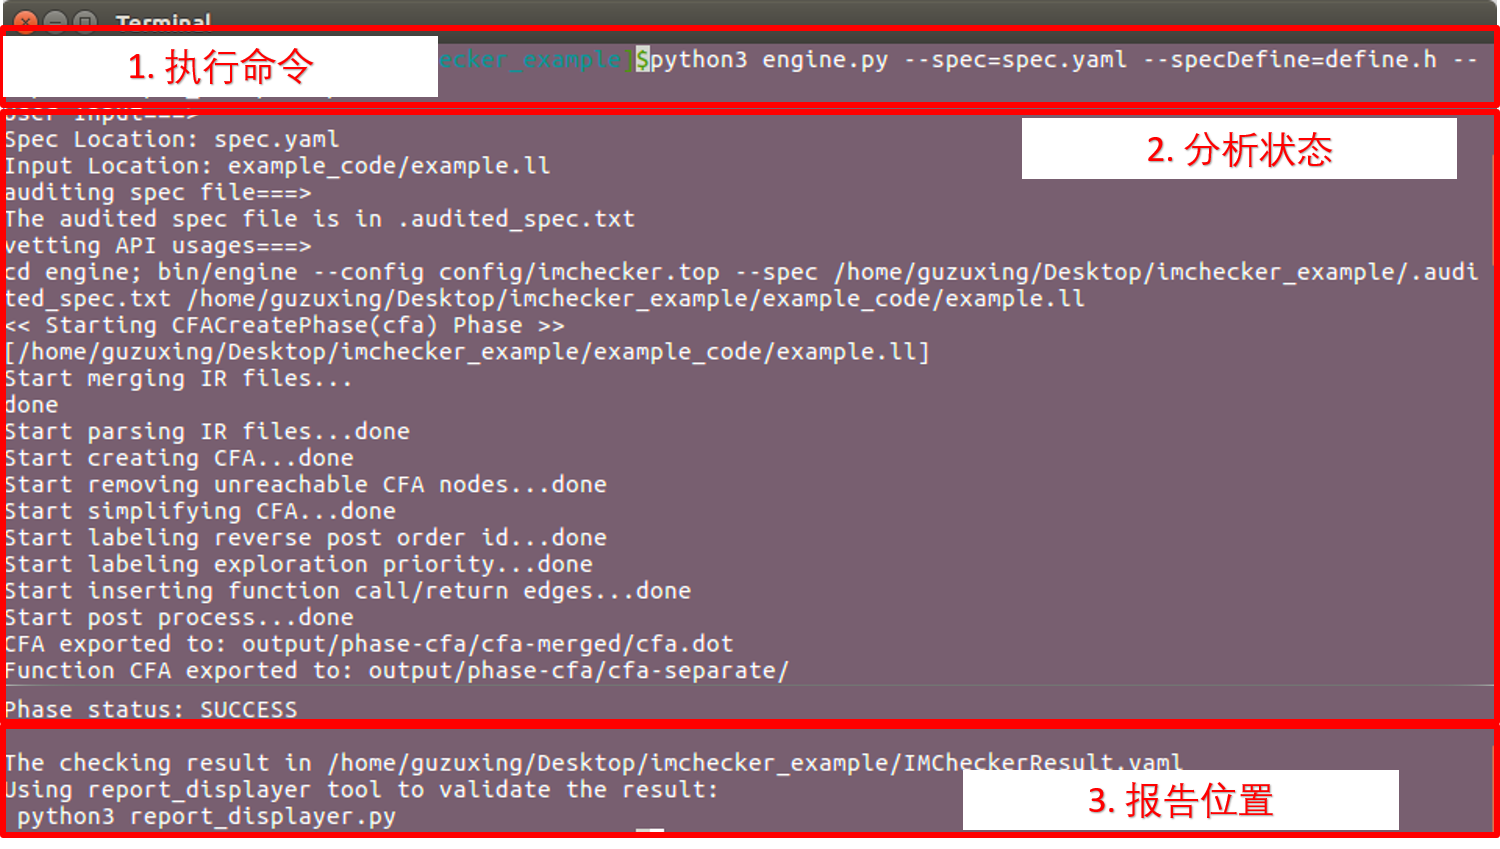
\includegraphics[width=0.85\linewidth]{figures/cp4-IMChecker-engine.png}
	\caption{
		IMChecker分析引擎运行时截图。
	}
	\label{fig:4-3-IMChecker-engine}
\end{figure}

研究人员和工具开发人员通过简单易用的用户接口,
以提高工具的实用性,减轻使用者的负担。
特别地,每个工具针对自己应用对象的不同,在工具接口上都有自己的设计目的和特定。
本文通过对IMChecker方法的实现和封装,以命令行的方式帮助开发者,
直接调用分析引擎,并生成对应的缺陷分析报告。

如图~\ref{fig:4-3-IMChecker-engine}所示,IMChecker分析引擎在命令行中通过直接调用如下指令即可运行,
\begin{lstlisting}[language={bash},
basicstyle=\linespread{0.8}\listingsfont,
numbers=none,
xleftmargin=.1\textwidth]
(*@\textcolor{blue}{Ubuntu@~:Python3}@*) engine.py --spec=XXX --specDefine=XXX --input=XXX
\end{lstlisting}
其中,参数的具体含义如下:
\begin{itemize}
	\item spec: 目标接口使用约束IMSpec文件。该文件可以由IMSpec规约撰写工具生成,也可以用户直接根据IMSpec语法进行撰写。其内容如图~\ref{fig:2-4-example-imspec}中IMSpec实例所示。
	\item specDefine: 规约实例中宏参数的具体定义。在分析阶段,分析引擎会根据宏定义,对IMSpec规约进行展开,以及缺陷检测。
	例如在上文介绍的define.h文件。
	\item input: 待分析文件。目前分析引擎在单独使用时,
	接受单独可编译的C源代码,以及预处理后的LLVM-IR中间表达。
	在Tsmart工具集中,我们提供了Build-capture编译抓取工具,
	自动生成LLVM-IR表达。使用者亦可以通过Clang对项目进行编译,通过-S指令生成LLVM-IR表达。
	如果用户通过Tsmart项目对接口缺陷进行检测,则不需要考虑预处理操作。
	详细使用说明,可以参考Tsmart用户手册~\cite{tsmart}。
\end{itemize}
在分析过程中,IMChecker分析引擎将运行时状态输出到控制台中,以帮助开发者获知分析进展。
同时,对于分析中遇到的问题,开发者可以获知原因,并进行修复。
如图~\ref{fig:4-3-IMChecker-engine}所示,分析引擎首先对IMSpec规约文件进行解析,
接着进入预处理阶段创建CFA、分析阶段,最后针对于分析结果输出到缺陷检测结果报告IMCheckerResult.yaml中。

\begin{figure}[t]
	\centering
	\begin{minipage}{0.7\linewidth}
\begin{lstlisting}[language={C},
basicstyle=\linespread{0.7}\listingsfont,
numbers=none,frame=trBL,
xleftmargin=0pt]
  - (*@\textcolor{blue}{Bug}@*):
    (*@\textcolor{blue}{API}@*): fopen
    (*@\textcolor{blue}{Type}@*): IPC
    (*@\textcolor{blue}{Spec}@*):  fopen==> fopen_arg1!=NULL
    (*@\textcolor{blue}{Reason}@*): Missing or incorrect validation of parameter
    (*@\textcolor{blue}{Error}@*): 
      - IMChecker/tools/example_code/example.c:bad1:14
    (*@\textcolor{blue}{Good}@*): 
      - IMChecker/tools/example_code/example.c:good1:52
\end{lstlisting}
	\end{minipage}
	\caption{
		IMChecker分析结果示例。
	}
	\label{fig:4-3-Result}
\end{figure}

IMChecker分析引擎将结果输出到缺陷检测报告中,针对每一个目标API的一种缺陷模式,
缺陷检测结果将汇总在一个“Bug”标签中。
图~\ref{fig:4-3-Result}中给出了图~\ref{fig:2-4-example}中程序检测的一个缺陷实例,其中
\begin{itemize}
	\item Bug标签为一个目标API某一种缺陷的分类符。
	\item API标签给出了目标API的接口名。
	\item Type标签给出缺陷的具体类型。在实际应用场景中,本文将缺陷的类型进行进一步扩展,以展示更具体的缺陷原因。
	\item Spec标签给出了导致误用的具体约束条件。例如图说所描述的是,第一个参数不可以为NULL。
	\item Reason标签给出基于自然语言的缺陷原因。
	\item Error标签给出具体缺陷发生的程序位置。
	\item Good标签给出针对于目标API正确使用的程序位置,即满足约束的位置。
\end{itemize}
如果,该类型的错误存在多个或者存在多个正确的使用,则Error和Good标签拥有多个实例。
使用者可以通过缺陷检测结果报告对缺陷进行核对,也可以通过IMDisplayer工具进行分析。
此外,该缺陷报告也可以供其他工具的开发者利用。


\subsection{结果展示模块}
\begin{figure}[t]
	\centering
	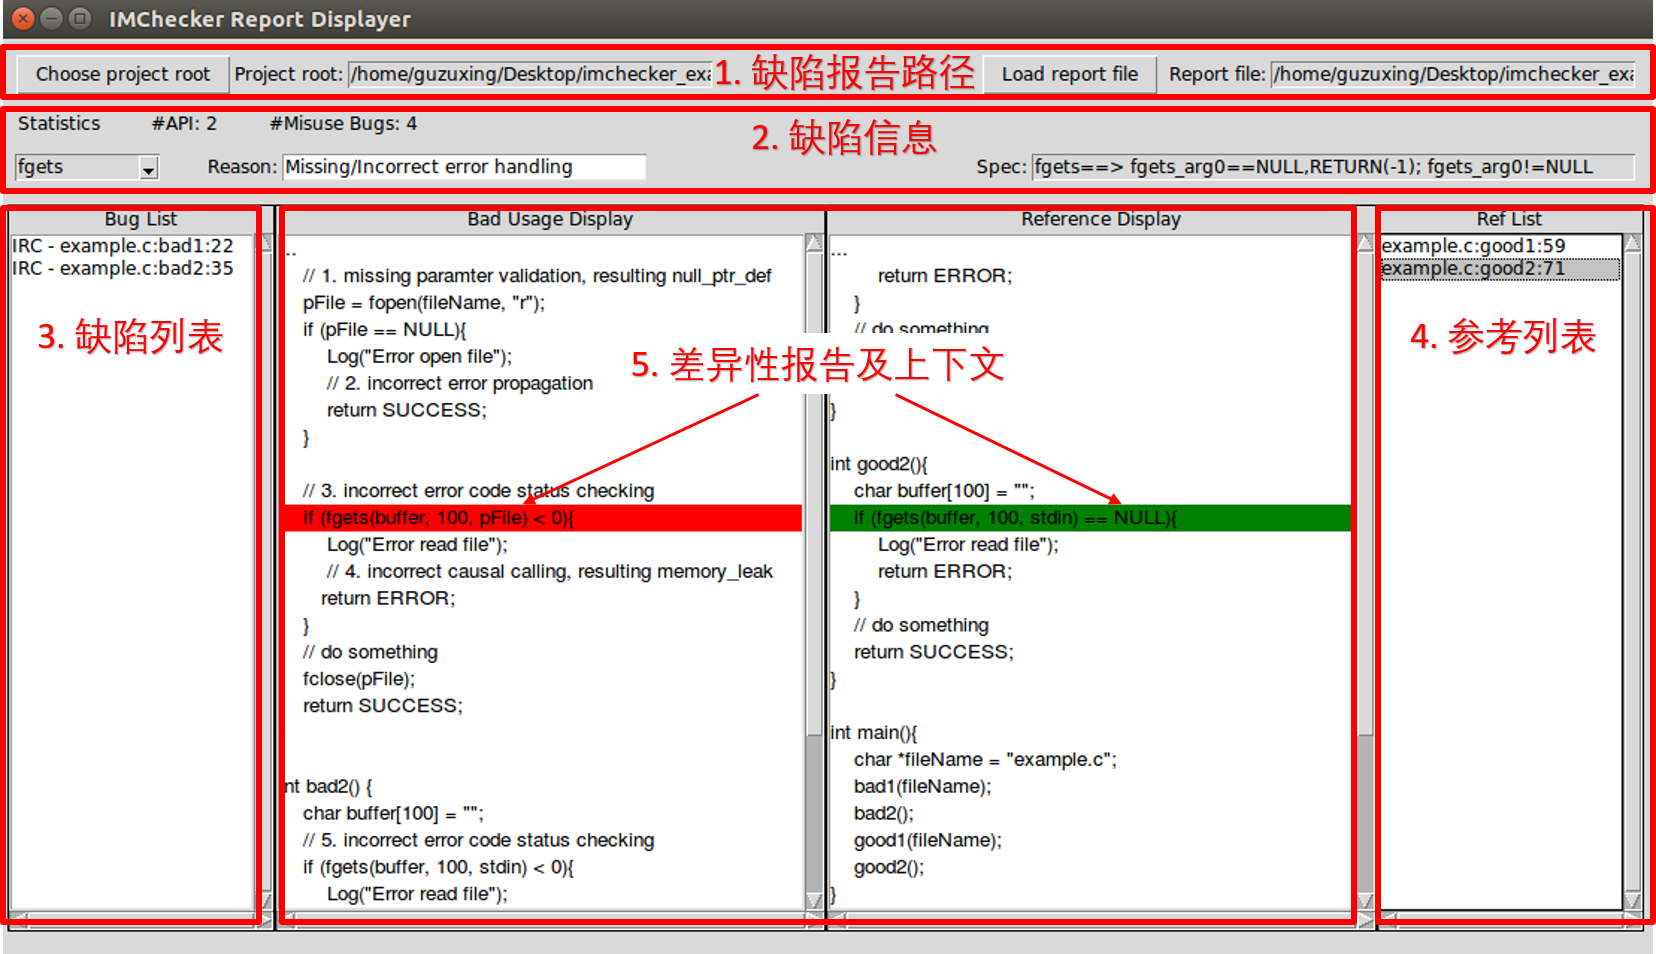
\includegraphics[width=0.85\linewidth]{figures/cp4-IMDisplayer.png}
	\caption{
		IMDisplayer结果展示工具运行时截图。
	}
	\label{fig:4-3-IMDisplayer}
\end{figure}

为了更好的对缺陷结果进行展示,研究人员和开发者设计并实现了各种各样的GUI界面。
针对于接口使用和接口缺陷的特点,本文设计了本文设计了IMDisplayer结果展示工具,
通过差异性结果对比的方式,帮助开发者深入理解API使用上下文的不同,
并未开发者修复缺陷提供参考。

IMDisplayer结果展示工具在命令行中通过直接调用如下指令即可运行,
\begin{lstlisting}[language={bash},
basicstyle=\linespread{0.8}\listingsfont,
numbers=none,
xleftmargin=.3\textwidth]
(*@\textcolor{blue}{Ubuntu@~:Python3}@*) report_displayer.py
\end{lstlisting}
如图~\ref{fig:4-3-IMDisplayer}所示,IMDisplayer工具包含五个部分:
缺陷报告路径选择模块、缺陷信息展示模块、缺陷列表、参考列表以及差异性报告及上下文信息。
用户在使用该工具时,首先要选择缺陷报告的路径信息。
基于缺陷报告,IMDisplayer工具会自动统计缺陷报告中的缺陷实例,
并将误用API数目、缺陷实例数目展示在界面上。
用户通过下拉菜单选择目标API,如图中所示,目标接口为\texttt{fgets()}函数。
在用户选择目标API后,IMDisplayer工具会更新左侧的缺陷列表,以展示该接口所有误用的情况。
此后,用户可以通过点击左侧的缺陷列表选择具体要审查的缺陷实例。
在用户进行选择后,IMDisplayer会更新缺陷实例的原因、违反的约束,以及右侧参考列表。
用户可以通过对参考列表中的使用实例进行选择,在缺陷展示框中,对缺陷和正确使用进行差异性对比。
例如图中红色和绿色为缺陷发生的位置和对应的正确使用的位置。

IMDisplayer的设计动机来源于两点:
(1)IMSpec有效性评估结果显示,相对于自然语言,IMSpec规约描述语言对接口使用约束描述更加有效,
即开发者更容易或者使用约束的条件。
因此,作者将缺陷所违反的IMSpec具体的约束展示在界面中,帮助开发者理解缺陷发生的原因。
(2)在应用阶段,开发者提交缺陷报告给对应的开发者。
最初,只提供了缺陷发生的原因和路径信息。
开发者则表示,如果能提供过多的语义信息,有助于理解缺陷的原因。
因此,作者扩展了缺陷分析引擎IMChecker,并设计了IMDisplayer工具。
特别地,在分析过程中,将正确使用的路径进行记录。
在IMDisplayer中,通过差异性比对的方式,展现缺陷和正确使用代码片段。
不仅有效的帮助使用者理解缺陷的原因,同时提供了缺陷修复的参考代码。
(3)IMDisplayer独立于分析引擎,通过解析缺陷报告中的标签来展示。
因此该工具能够扩展到其他应用场景。

\section{案例应用}
\label{sec:4.4}
本文的工作旨在对实际项目中C程序接口缺陷进行检测,以提高代码质量,应对现代软件开发的迫切需求。
因此,本章将Tsmar-IMChecker工具应用于广泛使用的开源项目中。
本小结将对应用对象和方法进行介绍,并总结应用的结果。
最后本小结讨论实际应用中的发现和不足,
为研究人员和开发人员进一步工作提供思路。

\subsection{实验准备}
\paragraph{应用对象}
作者选取三个典型领域的程序作为应用对象,评估Tsmar-IMChecker工具在实际项目中的有效性。
包括操作系统Linux内核、广泛使用的第三方库OpenSSL安全库和
使用了第三方库的应用软件。
其中,应用软件为Ubuntu16.04中,使用了OpenSSL安全库实现的应用软件。
Ubuntu系统提供了多个版本的OpenSSL安全库的实现,本文采用libssl1.0.0\footnote{https://packages.ubuntu.com/xenial/libssl1.0.0}作为应用对象。

应用软件的选择步骤如下。
首先,本文通过Ubuntu系统提供的软件包依赖管理工具所搜所有使用了libssl1.0.0的应用软件,即通过如下命令,
\begin{lstlisting}[language={bash},
basicstyle=\linespread{0.8}\listingsfont,
numbers=none,
xleftmargin=.25\textwidth]
(*@\textcolor{blue}{Ubuntu@~:}@*) apt-cache rdepends libssl1.0.0
\end{lstlisting}
\texttt{apt-cache rdepends}命令\footnote{http://manpages.ubuntu.com/manpages/bionic/man1/apt-rdepends.1.html}
能够查看一个软件包被哪些软件包所依赖。
搜索的结果显示,超过1200应用软件包依赖于libssl1.0.0。
接着,对于这些软件包,作者在Github中搜索是否存在这些软件包。
目的在于,确保这些应用对象然而活跃于开源社区中,同时提交的缺陷报告可以及时获得回复。
对于软件包编译、分析需要大量的时间,
因此本文选择了15个广泛使用、不同应用领域、开发者持续维护的应用软件。
为了有效评估Tsmar-IMChecker的检测能力,所有应用对象选择了截止至2018年7月10-15日的最新的稳定版本,
即Linux内核4.18-rc4,OpenSSL-1.1.1-pre8,以及Ubuntu操作系统中应用软件:
\begin{itemize}
	\item dma: 邮件服务,主分支,86个关注(Star数目)
	\item exim: 邮件服务,版本4.91,393个关注
	\item hexchat: 网络实时聊天,版本2.14.1,1949个关注
	\item httping: 针对HTTP请求的Ping服务,主分支,302个关注
	\item ipmitool: 针对智能平台管理接口(Intelligent Platform Management Interface,IPMI)的控制系统,主分支,122个关注
	\item open-vm-tools: WMware软件管理,版本10.3.0,956个关注
	\item irssi: 通信软件,版本1.1.1,1918个关注
	\item keepalive: 负载均衡管理软件,版本2.0.5,1717个关注
	\item thc-ipv6: IPV6攻击测试软件,主分支,442个关注
	\item freeradius-server: 多协议服务器,主分支,943个关注
	\item trafficserver: 网络代理服务器,版本7.1.3,907个关注
	\item tinc: VPN后台服务,版本1.1-pre16,854个关注
	\item sslplit: SSL/TLS攻击测试工具,主分支,1106个关注
	\item rdesktop: 远程桌面服务,主分支,577个关注
	\item proxytunnel: 网络代理服务,主分支,155个关注
\end{itemize}

\paragraph{目标API}
目标API包括两个部分。
(1)针对于Linux内核和OpenSSL,本文将第~\ref{sec:2.5}节中撰写的IMSpec约束,作为目标API。
旨在通过这些被误用过的API再次对这些项目进行检测,以观察是否依旧存在误用情况。
(2)对于15个Ubuntu中的应用软件,本文首先通过GNU cflow\footnote{http://www.gnu.org/software/cflow/}抽取这些应用软件的函数调用图。
基于函数调用图和OpenSSL提供的用户手册,选择调用图中使用的OpenSSL中的接口。
例如在dma项目中,通过cflow和OpenSSL用户手册的结果,
我们发现该项目使用了OpenSSL中包含\texttt{SSL\_connect()}等17个不同的API。
接着在15个项目中,本文将提取的API的使用情况进行总结,选取至少使用过两次的接口。
最终共选择78个不同的API作为检测目标。
本文将这些目标API的IMSpec规约描述文件公开\footnote{https://github.com/tomgu1991/IMChecker/tree/master/imspec},共研究人员和开发者使用。

\paragraph{实验环境}
本文在一台装有64 位Ubuntu 16.04的台式机上进行实验。
该机器配有Intel(R) Core(R) i5-3470@3.20GHz-4核心CPU和32GB内存。
Tsmart-IMChecker工具需要通过Clang对项目进行预处理,抽取LLVM-IR的中间表达。
然而,部分项目无法完全被Clang支持,例如Linux内核。
同时,部分项目依赖于旧版本的编译环境或者其他编译库难以满足。
这对于这些情况,本文工作人工的方式,对这些目标项目中使用了目标API的文件进行单独编译。
并将这些能够编译的文件作为分析目标,提供给分析引擎。
为了控制分析的时间和输出结果,本文每次分析执行一个目标API。
所有的分析中,本文以3小时作为时间界限,即如果三小时无法完成,则将已有分析结果输出。
对于所有找到的实际缺陷,本文作者在对象项目中提交缺陷报告或者提交修改申请(Pull Request)。

\subsection{缺陷检测结果}
%https://github.com/tomgu1991/IMChecker/blob/master/evaluation_data/new_bugs/bug_list.md
\begin{table}[b]
	\centering
	\begin{minipage}[t]{0.7\linewidth} % 如果想在表格中使用脚注,minipage是个不错的办法
		\caption{Tsmart-IMChecker实际项目应用结果}
		\label{tab:4-4-result}
		\begin{tabular}{cccc}
			\hline
			项目名称 & 缺陷报告总数 & 确认未修复 & 已经修复 \\
			\hline
			Linux内核 & 30 & 20 & 5 \\
			 OpenSSL & 17 & 5 & 12\\
			  dma  & 1 & 0 & 1\\
			   exim   &2  & 0 & 2\\
			    hexchat    & 2 & 1 & 0\\
			   httping & 1 & 1 & 0\\
			   ipmitool  & 1 & 1 & 0\\
			    open-vm-tools   &2  & 0 & 2\\
			     irssi    & 2 & 1 & 0\\
			 keepalive & 2 & 0 & 2\\
			 thc-ipv6 & 2 & 0 & 2\\
			 freeradius-server & 2 & 0 & 2\\
			 trafficserver & 3 & 0 & 0\\  
			  tinc  & 2 & 0 & 2\\
			   sslplit   & 2 & 0 & 2\\
			   rdesktop     & 2 & 0 & 0\\
			      proxytunnel    & 2 & 0 & 0\\
			      总计 & 75 & 29 & 32 \\
			\hline
		\end{tabular}
	\end{minipage}
\end{table}
Tsmart-IMChecker工具针对于上述17个开源项目的应用结果如表~\ref{tab:4-4-result}所示。
在第一列中,给出了项目的名称。
在第二列中,对缺陷报告总数进行展示。
第三列和第四列分别给出在报告的缺陷中,开发者已经确认但没有修复的个数,
以及开发者确认并且修复的缺陷报告个数。
在所有检测的结果中,本文作者过滤后
在17个项目中共提交了75个实际接口误用缺陷。
其中Linux内核具有30个,25个已经被开发者确认,5个已经在最新的代码中进行修复与集成。
OpenSSL共检测出17个缺陷,全部被开发者确认,其中12个已经被修复并集成到主分支和发布版本中。
Ubuntu系统中的应用软件分别检测到1-3个缺陷,每个项目具体数据如表中所示。
综合来看,75个缺陷中,61个已经被开发者确认,32个已经被成功修复。
下文将对Linux内核、OpenSSL和Ubuntu中的应用软件中的缺陷进行详细讨论。

\begin{table}[!b]
	\centering
	\scriptsize
	\setlength{\tabcolsep}{4.25pt}
	\begin{minipage}[t]{0.97\linewidth} % 如果想在表格中使用脚注,minipage是个不错的办法
		\caption{Linux内核-4.18rc4缺陷检测结果}
		\scriptsize
		\label{tab:4-4-linux}
		\begin{tabular}{ccclcc}
			\hline
			\multirow{2}{*}{编号}& 缺陷 & \multirow{2}{*}{误用API} & \multicolumn{1}{c}{文件位置} & 缺陷 & \multirow{2}{*}{状态\footnote{$\checkmark\checkmark$为已经修复的缺陷,$\checkmark$为确认的缺陷,$P$为未确认的缺陷。}} \\
			& 编号 & & \multicolumn{1}{c}{文件名:调用函数} & 种类 & \\
			\hline
1 & 200489 & kzalloc & tlb\_uv.c: \textbf{init\_per\_cpu} & ICC & \checkmark \\
2 & 200505 & alloc\_disk & pktcdvd.c: \textbf{pkt\_setup\_dev}& IEH & \checkmark\checkmark \\
3 & 200511& kzalloc & clk-pxa.c: \textbf{clk\_pxa\_cken\_init} & ICC & \checkmark \\
4 & 200519& devm\_clk\_get & hci\_bcm.c: \textbf{bcm\_get\_resources} & IPU & \checkmark \\
5 & 200521& kzalloc & ip22-gio.c: \textbf{ip22\_check\_gio} & ICC & \checkmark \\
6 & 200533& nla\_nest\_start & ncsi-netlink.c: \textbf{ncsi*\_nl}& IPU & \checkmark\checkmark \\
7 & 200535 & nla\_nest\_start & conntrack.c: \textbf{ovs*\_get}& IPU & \checkmark\checkmark \\
8 & 200537 & nla\_nest\_start & datapath.c: \textbf{queue*\_packet} & IPU & \checkmark \\
9 & 200539 & alloc\_skb & chtls\_cm.c: \textbf{chtls*\_conn} & ICC & \checkmark \\
10 & 200541 & \_\_send*alloc\_skb & team.c: \textbf{team\_*\_get} & ICC & \checkmark \\
11 & 200543 & devm\_kzalloc & gpio-tegra.c: \textbf{tegra\_gpio\_probe}& IEH & \checkmark \\
12 & 200545 & devm\_kzalloc & core.c: \textbf{rsnd\_probe}& IEH & \checkmark \\
13 & 200547 & devm\_kzalloc & atmel*\_output.c: \textbf{atmel\_*\_endpoint} & ICC & $P$ \\
14 & 200549 & pci*ext\_capability & nic\_main.c: \textbf{pci*\_capability} & IPU & \checkmark \\
15 & 200551 & pci*ext\_capability & dpc.c: \textbf{dpc\_probe} & IPU & \checkmark\checkmark \\
16 & 200555 & devm*init\_i2c & hmc5843\_i2c.c: \textbf{hmc5843*\_probe} & IPU & \checkmark \\
17 & 200557 & devm\_ioremap & pata\_pxa.c: \textbf{pxa\_ata\_probe} & IEH & \checkmark \\
18 & 200559 & alloc\_workqueue & fm10k\_main.c: \textbf{fm10k*\_module} & ICC & \checkmark \\
19 & 200561 & ida\_pre\_get & namespace.c: \textbf{mnt*\_id} & IPU & \checkmark\checkmark \\
20 & 200563 & wm831x*\_read & clk-wm831x.c: \textbf{wm831x*prepared} & IEH & \checkmark \\
21 & 200565 & dma\_mapping\_error & qib\_sdma.c: \textbf{qib*send} & IEH & \checkmark \\
22 & 200567 & get\_zeroed\_page & sysinfo.c: \textbf{sysinfo\_show} & IEH & \checkmark \\
23 & 200569 & kzalloc & mach-mx27ads.c: \textbf{mx27ads*\_init} & ICC & $P$ \\
24 & 200571 & kzalloc & board-v7.c: \textbf{i2c\_quirk} & ICC & \checkmark \\
25 & 200573 & kzalloc & coherency.c: \textbf{armada\_*\_init} & ICC & \checkmark \\
26 & 200575 & kzalloc & octeon-irq.c: \textbf{octeon*\_map} & ICC & \checkmark \\
27 & 200577 & kzalloc & gptu.c: \textbf{clkdev*\_gptu} & ICC & $P$ \\
28 & 200579& kzalloc & octeon-irq.c: \textbf{octeon*\_map} & ICC & $P$ \\
29 & 200581 & kzalloc & sysctrl.c: \textbf{clkdev\_add\_pci} & ICC  & $P$ \\
30 & 200583 & kzalloc & msi-xlp.c: \textbf{xlp*\_irqs} & ICC & \checkmark \\
			\hline
		\end{tabular}
	\end{minipage}
\end{table}

\paragraph{Linux内核}
如表~\ref{tab:4-4-linux}中所示,在Linux内核中,
Tsmart-IMChecker工具共提交30个未被报告的接口缺陷。
针对于每一个缺陷报告,本文作者首先在Linux的缺陷报告系统\footnote{https://bugzilla.kernel.org}中进行查询,
是否已经有开发者进行提交。
如果没有,则对缺陷报告进行提交。
在提交报告给开发者后,其中25个已经被开发者确认并收到开发者回复的邮件。
针对于维护者的要求,本文作者正在提交相应的修改记录。
其中5个已经被维护者接受,2个已经集成到Linux最新版当中,3个在进行代码风格修改。

\begin{figure}[t]
	\centering
	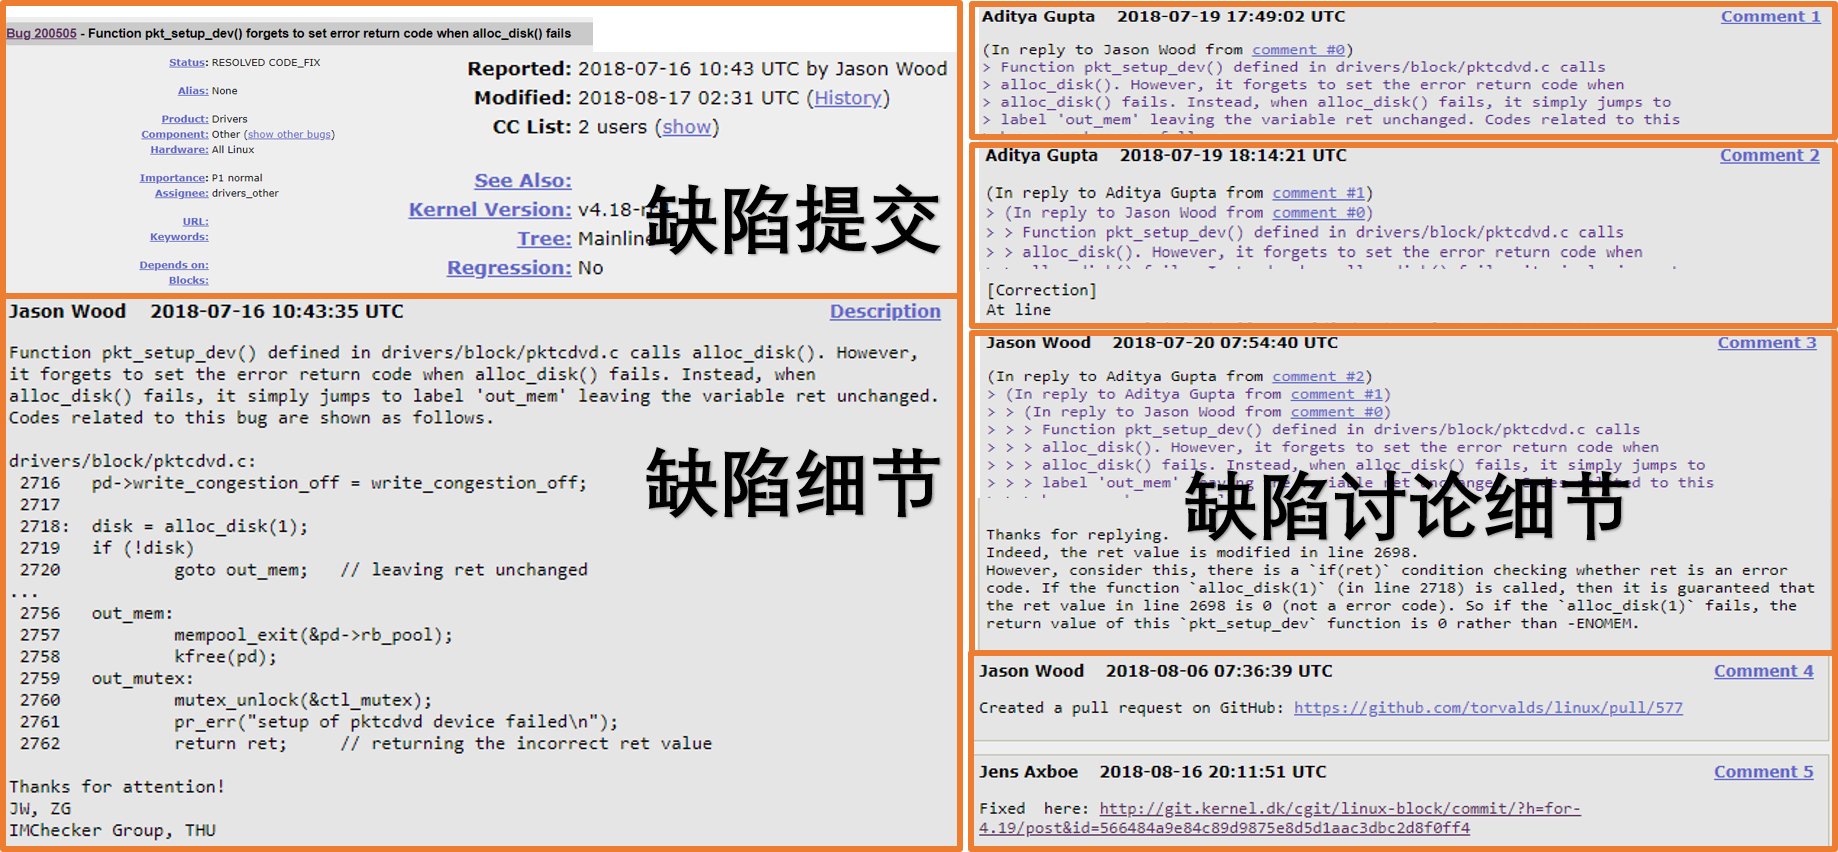
\includegraphics[width=\linewidth]{figures/cp4-linux-example.png}
	\caption{
		Linux接口缺陷200505提交和讨论记录。
	}
	\label{fig:4-4-linux-example}
\end{figure}

\begin{figure}[t]
	\centering
	\begin{lstlisting}
(*@\textcolor{black}{"summary": "fix setting of 'ret' error return for a few cases",}@*)
"date": "2018-08-16",
"author": "Jens Axboe",
drivers/block/pktcdvd.c
=======================================================
@@ -2740,6 +2740,7 @@ static int pkt_setup_dev(dev_t dev, dev_t* pkt_dev)
pd->write_congestion_on  = write_congestion_on;
pd->write_congestion_off = write_congestion_off;

+	ret = -ENOMEM;
	disk = alloc_disk(1);
	if (!disk)
		goto out_mem;
	\end{lstlisting}
	\caption{
		Linux接口缺陷200505修复细节。
	}
	\label{fig:4-4-linux-example-fix}
\end{figure}


如图~\ref{fig:4-4-linux-example}为作者将误用接口\texttt{alloc\_disk()}的缺陷实例提交,以及修复的记录截图。
根据Linux中错误处理机制,接口\texttt{alloc\_disk()}出错时,外层调用者需要返回\textbf{-ENOMEM}来表示内存不足的错误信息。
然而在drivers/block/pktcdvd.c文件的\texttt{pkt\_setup\_dev()}函数中的2718行调用该接口后,
在异常检测路径上并有对返回值机型修改,导致一个不正确的异常处理缺陷(IEH)。
在对该缺陷进行仔细核对后,本文作者将缺陷提交到Linux缺陷报告系统中,编号为200505。
该缺陷报告在提交后,获得了维护者的回复。
在经过三轮的缺陷细节讨论过后,该缺陷被维护者确认,并集成到Linux内核的主分支中。
缺陷修复的细节如图~\ref{fig:4-4-linux-example-fix}中所示,
即在返回之前对返回值赋值为的错误代码\textbf{-ENOMEM}。


\paragraph{OpenSSL}
\begin{table}[!b]
	\centering
	\scriptsize
	\setlength{\tabcolsep}{4.25pt}
	\begin{minipage}[t]{0.97\linewidth} % 如果想在表格中使用脚注,minipage是个不错的办法
		\caption{OpenSSL-1.1.1-pre8缺陷检测结果}
		\scriptsize
		\label{tab:4-4-openssl}
		\begin{tabular}{ccclcc}
			\hline
			\multirow{2}{*}{编号}& 缺陷 & \multirow{2}{*}{误用API} & \multicolumn{1}{c}{文件位置} & 缺陷 & \multirow{2}{*}{状态\footnote{$\checkmark\checkmark$为已经修复的缺陷,$\checkmark$为确认的缺陷。}} \\
			& 编号 & & \multicolumn{1}{c}{文件名:调用函数} & 种类 & \\
			\hline
1 & 6567 & RAND\_bytes & speed.c: \textbf{RAND*\_loop} & IEH & \checkmark\checkmark \\
2 & 6568 & ASN1\_INTEGER\_get & tasn\_utl.c: \textbf{asn1\_do\_adb} & IPU & \checkmark \\
3 & 6569& ASN1\_INTEGER\_set & p12\_init.c: \textbf{PK*init} & IPU & \checkmark\checkmark \\
4 & 6570& ASN1\_object\_size & asn1\_gen.c: \textbf{generate\_v3 } & IEH & \checkmark \\
5 & 6572& BN\_set\_word & t1\_lib.c: \textbf{ssl*\_dh} & IEH & \checkmark\checkmark \\
6 & 6573& HMAC\_Init\_ex & apps/speed.c: \textbf{HMAC\_loop} & IEH & \checkmark \\
7 & 6574 & EVP\_PKEY\_get0\_DH & statem\_srvr.c: \textbf{tls*\_dhe} & IPU & \checkmark\checkmark \\
8 & 6575 & EC\_KEY\_generate\_key & speed.c: \textbf{run\_benchmark} & IEH & \checkmark \\
9 & 6781 & EC*new*\_name & ec\_ameth.c: \textbf{eckey\_type2param} & ICC & \checkmark\checkmark \\
10 & 6789 & ASN1\_INTEGER\_set & v3\_tlsf.c: \textbf{v2i*FEATURE} & IEH & \checkmark\checkmark \\
11 & 6820 & ASN1\_INTEGER\_to\_BN & ts\_lib.c: \textbf{TS*\_bio} & IPU & \checkmark\checkmark \\
12 & 6822 & BN\_sub & rsa\_ossl.c: \textbf{rsa*\_encrypt} & IEH & \checkmark\checkmark \\
13 & 6973 & EVP\_MD\_CTX\_new & ocsp\_srv.c: \textbf{OCSP*\_sign} & IPU & \checkmark\checkmark \\
14 & 6977 & ASN1\_INTEGER\_set & pk7\_lib.c: \textbf{PKCS7*type} & IEH & \checkmark\checkmark \\
15 & 6982 & OBJ\_nid2obj & asn\_moid.c: \textbf{do\_create} & IEH & \checkmark\checkmark \\
16 & 6983 & BN\_sub & bn\_x931p.c: \textbf{BN*\_Xpq} & IEH & \checkmark\checkmark \\
17 & 7235 & DH\_set0\_key & dh\_lib.c: \textbf{DH*\_key} & IEH & \checkmark \\
			\hline
		\end{tabular}
	\end{minipage}
\end{table}

如表~\ref{tab:4-4-openssl}中所示,在OpenSSL中,Tsmart-IMChecker工具共提交17个未被报告的接口缺陷。
针对于每一个缺陷报告,本文作者首先在Github中OpenSSL代码库中提交Issue。
在提交报告给开发者后,所有的缺陷报告都获得了开发者的回复。
其中12个已经被维护者修复并集成在主分支内,5个被标记为待评估(Assessed)。
OpenSSL与Linux内核的缺陷报告系统不同,基于Github的Issue系统维护。
因此,缺陷的提交和修复往往能够获得及时的反馈。

\begin{figure}[t]
	\centering
	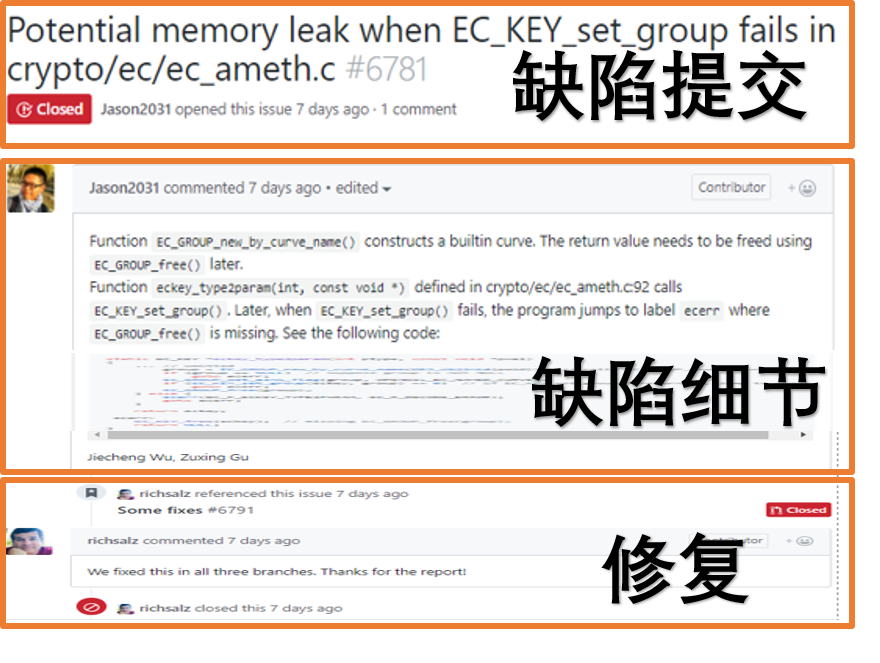
\includegraphics[width=0.8\linewidth]{figures/cp4-openssl-example.png}
	\caption{
		OpenSSL缺陷6781提交和修复记录。
	}
	\label{fig:4-4-openssl-example}
\end{figure}

图~\ref{fig:4-4-openssl-example}是作者在OpenSSL项目检测到的一个内存泄漏缺陷。
OpenSSL设计了\texttt{EC\_GROUP\_new\_by\_curve\_name()}来创建EC\_GROUP对象。
该对象在声明周期结束后需要通过\texttt{EC\_GROUP\_free()}进行释放。
然而在ec\_ameth.c文件的\texttt{eckey\_type2param()}中,在一条错误路径上,
开发者并没有进行释放,导致一个内存泄漏错误。
如图~\ref{fig:4-4-openssl-example-fix}中所示,
开发者在12行进行了内存对象的申请,然而在16行的if判断错误处理中,
直接通过goto语句跳转到21行继续执行。
因此这条异常处理路径上,忽视了对于12行申请的内存对象\texttt{group}的释放。
在作者提交缺陷报告,并说明出错路径后,开发者在12小时内完成修复。
修复细节如图~\ref{fig:4-4-openssl-example-fix}所示。
OpenSSL项目设计了明确的错误代码机制,并在用户手册中提供基于自然语言的描述。
然而,项目的开发者却忽略了大量的异常处理检测。
例如,缺陷6569、6572、6798和6982,均由不正确的异常处理原因,导致的软件缺陷。
作者在提交缺陷报告后,开发者均进行了相应的修复。


\begin{figure}[t]
	\centering
	\begin{lstlisting}
(*@\textcolor{black}{"summary": "Avoid memory leak on failure path.Thanks to Jiecheng Wu, Zuxing Gu for the report.",}@*)
"date": "2018-07-26",
"author": "richsalz",
=======================================================
@@ -122,13 +122,12 @@ static TLS_FEATURE *v2i_TLS_FEATURE(const X509V3_EXT_METHOD *method,
+   EC_GROUP *group = NULL;
	[...]
	else if (ptype == V_ASN1_OBJECT) {
		const ASN1_OBJECT *poid = pval;
-		EC_GROUP *group;
		[...]
		group = EC_GROUP_new_by_curve_name(OBJ_obj2nid(poid));
		if (group == NULL)
			goto ecerr;
		EC_GROUP_set_asn1_flag(group, OPENSSL_EC_NAMED_CURVE);
		if (EC_KEY_set_group(eckey, group) == 0)
			goto ecerr;
		EC_GROUP_free(group);
	} else {
	[...]
ecerr:
	EC_KEY_free(eckey);
+	EC_GROUP_free(group);
	return NULL;
	\end{lstlisting}
	\caption{
		OpenSSL缺陷6781修复细节
	}
	\label{fig:4-4-openssl-example-fix}
\end{figure}

\paragraph{应用程序}
\begin{table}[!t]
	\centering
	\setlength{\tabcolsep}{2.25pt}
	\begin{minipage}[t]{\linewidth} % 如果想在表格中使用脚注,minipage是个不错的办法
		\caption{Ubuntu16.04应用软件缺陷检测结果}
		\label{tab:4-4-apps}
		\begin{tabular}{ccclcc}
			\hline
			 项目 & 缺陷 & \multirow{2}{*}{误用API} & \multicolumn{1}{c}{文件位置} & 缺陷 & \multirow{2}{*}{状态\footnote{$\checkmark\checkmark$为已经修复的缺陷,$\checkmark$为确认的缺陷,$P$为未确认的缺陷。}} \\
			名称 & 编号 & & \multicolumn{1}{c}{文件名:调用函数} & 种类 & \\
			\hline
dma & 59 & SSL\_connect & crypto.c: \textbf{smtp*\_crypto} & IEH & \checkmark\checkmark \\
\cline{1-1}
\multirow{2}{*}{exim} & 2316 & X509\_NAME\_oneline & tls-openssl.c: \textbf{x509*\_names} & IEH & \checkmark\checkmark \\
    & 2317 & SSL\_CTX*\_list & tls-openssl.c: \textbf{tls*\_cb} & IEH & \checkmark\checkmark \\
\cline{1-1}
\multirow{2}{*}{hexchat} & 2244 & BN\_set\_word & dh1080.c: \textbf{dh1080\_init} & IEH & \checkmark \\
    & 2245 & DH\_set0\_key & dh1080.c: \textbf{dh1080\_compute\_key} & IEH & $P$ \\
\cline{1-1}
\multirow{1}{*}{httping} & 41 & SSL\_CTX\_new & mssl.c: \textbf{initialize\_ctx} & ICC & \checkmark \\
\cline{1-1}
\multirow{1}{*}{ipmitool} & 37 & MD2\_Init & auth.c: \textbf{ipmi\_auth\_md2} & IEH & \checkmark \\
\cline{1-1}
\multirow{1}{*}{open-} & 291 & SSL\_*list & sslDirect.c: \textbf{SSL\_NewContext} & IEH & \checkmark\checkmark \\
vm-tools & 292 & X509*\_current\_cert & certverify.c: \textbf{VerifyCallback} & IPU & \checkmark\checkmark \\
\cline{1-1}
\multirow{2}{*}{irssi} & 943 & SSL*\_certificate & net*-openssl.c: \textbf{irssi*\_handshake} & IPU & $P$ \\
    & 944 & BIO\_read & certverify.c: \textbf{set*\_info} & IEH & \checkmark \\
\cline{1-1}
\multirow{2}{*}{keepalive} & 1003 & SSL*\_new & ssl.c: \textbf{build*\_ctx} & ICC & \checkmark\checkmark \\
    & 1004 & SSL\_new & ssl.c: \textbf{ssl\_connect} & ICC & \checkmark\checkmark \\
\cline{1-1}
\multirow{2}{*}{thc-ipv6} & 28 & BN\_new & thc-ipv6-lib.c: \textbf{thc\_memstr} & ICC & \checkmark\checkmark \\
    & 29 & BN\_set\_word & thc-ipv6-lib.c: \textbf{thc\_memstr} & IEH & \checkmark\checkmark \\
\cline{1-1}
\multirow{2}{*}{FreeRADIUS} & 2309 & BIO\_new & session.c: \textbf{tls*\_cert} & ICC & \checkmark\checkmark \\
    & 2310 & i2a\_ASN1\_OBJECT & session.c: \textbf{tls*\_cert} & IEH & \checkmark\checkmark \\
\cline{1-1}
\multirow{3}{*}{trafficserver} & 4292 & SSL\_CTX\_new & http\_load.c: \textbf{handle\_connect} & ICC & $P$ \\
    & 4293 & SSL\_new & http\_load.c: \textbf{handle\_connect} & ICC & $P$ \\
    & 4294 & SSL\_write & http\_load.c: \textbf{handle\_connect} & IEH & $P$ \\
\cline{1-1}
\multirow{2}{*}{tinc} & 205 & BN\_hex2bn & tincd.c: \textbf{keygen} & IPU & \checkmark\checkmark \\
    & 206 & RAND\_load\_file & tincd.c: \textbf{main} & IEH & \checkmark\checkmark \\
\cline{1-1}
\multirow{2}{*}{sslsplit} & 224 & SSL*\_certificate & pxyconn.c: \textbf{pxy*\_create} & IEH & \checkmark\checkmark \\
    & 225 & SSL*\_PrivateKey & pxyconn.c: \textbf{pxy*\_create} & IEH & \checkmark\checkmark \\
\cline{1-1}
\multirow{2}{*}{rdesktop} & 280 & BN\_bin2bn& ssl.c: \textbf{rdssl*\_encrypt} & IEH & $P$ \\
    & 281 & BN\_mod\_exp & ssl.c: \textbf{rdssl*\_encrypt} & IEH & $P$ \\
\cline{1-1}
\multirow{2}{*}{proxytunnel} & 36 & SSL\_connect & ptstream.c: \textbf{stream*\_ssl} & IEH & $P$ \\
    & 37 & SSL\_new& ptstream.c: \textbf{stream*\_ssl} & ICC & $P$ \\
			\hline
		\end{tabular}
	\end{minipage}
\end{table}

OpenSSL软件库是网络通信领域广泛使用的安全库,这些接口误用会极大地损害系统的可靠性。
因此,对OpenSSL项目中接口缺陷检测本身具有重要意义。
一方面,可以提高软件库本身的质量。
另一方面,通过完善软件库代码的质量,能够有效为使用者提供可靠的用例。
我们在Ubuntu16.04的应用软件中,对OpenSSL软件库接口缺陷进行检查,
并将28检测结果提交给对应的15个项目中。
如表~\ref{tab:4-4-apps}所示,28个缺陷中,18个被开发者接受,15个已经被成功修复。

\begin{figure}[t]
	\centering
	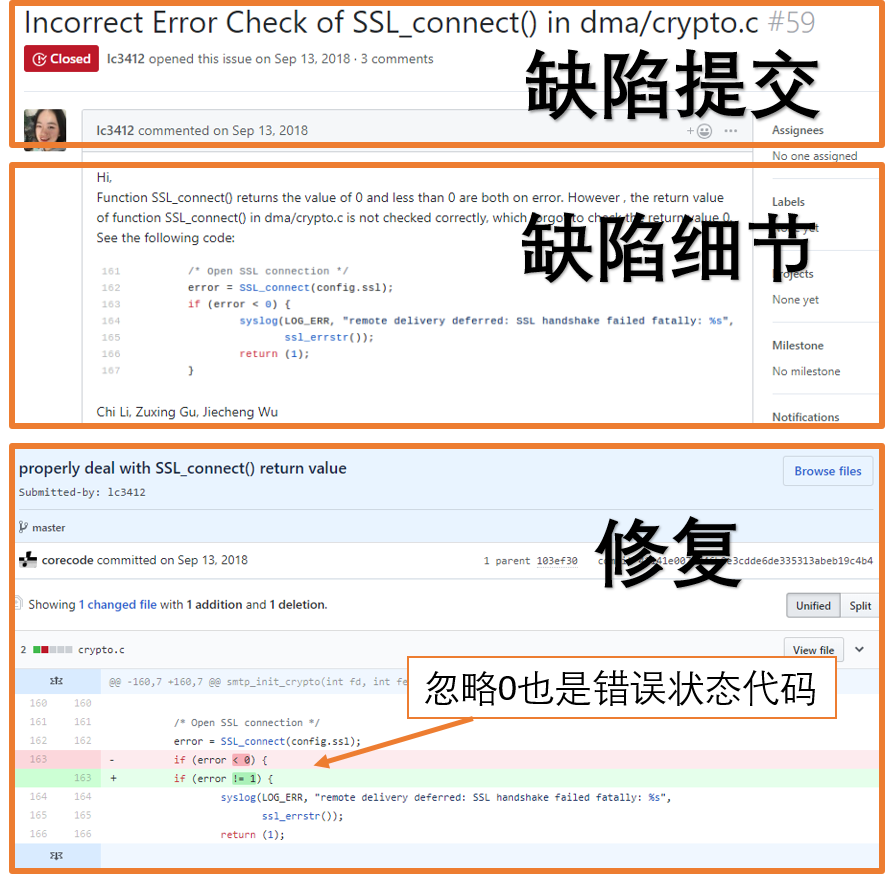
\includegraphics[width=0.8\linewidth]{figures/cp4-dma-example.png}
	\caption{
		dma缺陷59提交和修复记录。
	}
	\label{fig:4-4-dma-example}
\end{figure}

图~\ref{fig:4-4-dma-example}是作者在dma项目检测到的一个不正确的异常处理错误。
OpenSSL的官方用户手册中指出,\texttt{SSL\_connect()}函数用于初始化TSL/SSL服务器握手操作(handshake)。
根据TSL/SSL协议本身,当握手失败时,返回0代表链接被成功关闭,返回负数代表错误发生在协议层、链接等等。
所以该函数的异常处理需要考虑两种情况。
然而在dma项目中,开发者只对负数进行了检查,而忽略了0的情况。
导致项目的异常处理机制被破坏,如图中所示,没有正确的进行异常输出,返回对应的返回值。
本文作者在提交缺陷报告后,开发进行了对应的修复。
虽然有些项目对缺陷报告没有确认,但这些报告处于没有恢复的阶段,即开发者并没有否定检测结果为误报。
同时,相应的缺陷模式已经在其他的项目中获得认可。
因此本文认为,这些缺陷具有极高的可信度。


\subsection{应用经验总结}
本文将Tsmart-IMChecker应用于实际开源项目中,对接口缺陷进行分析,
并将缺陷报告提交给相应的开发者。
作者将缺陷检测、报告提交、开发者讨论和后续跟进工作中,
遇到的困难、总结的发现和项目应用经验总结下文中。
主要包括如下几个方面:
接口缺陷、现有文档、缺陷提交和开发者态度。

\paragraph{接口缺陷}
接口误用缺陷并不是个例,普遍存在于各种软件系统中。
特别地,本文共找到超过300个实际缺陷,并提交了75个高置信度的缺陷报告。
其中61个(81.33\%)被开发者接受,32个(42.67)已经被开发者修复。
一方面,
在本文分析之前,Linux内核和OpenSSL软件库作为广泛使用的基础软件,
两者代码已经被著名的分析工具(例如,商业工具Coverity~\cite{coverity}和学术工具Clang Static Analysis)检测过。
特别地,这些缺陷的目标API均从已有的缺陷修改记录中获得,
即这些缺陷已经在过去发生过。
然而,依旧存在大量的接口误用缺陷。
另一方面,被分析的应用软件中,每个都至少误用了一个OpenSSL的接口。
我们在后续的研究中,在其他的应用软件中发现了同样的现象。
在对缺陷模式、细节分析后,本文发现这些缺陷产生存在两方面的原因:
(1)软件库开发者间缺少缺陷报告分享机制。
开发者经常会忘记接口使用的约束。
特别地,即使新的代码中存在和过去发生的缺陷的模式一样,
并没有一个能够自动检测的方法,对开发者进行提示。
(2)客户端开发者缺少足够的领域知识,导致误用库函数。
即,客户端开发者在使用OpenSSL软件库时,没有深入理解或者参考文档,
导致接口使用错误。

总结来说,开发者在开发过程中,难免会产生接口误用,无论是无意忘记约束、缺少理解。
因此,Tsmart-IMChecker规模化、高效的分析工具对接口误用缺陷检测具有重要实际意义。
特别地,Tsmart-IMChecker基于规约描述语言进行检测,
容易扩展并集成领域知识。
同时可以渐进式的分析,即可以只应用于新修改的代码中。
\begin{figure}[b]
	\centering
	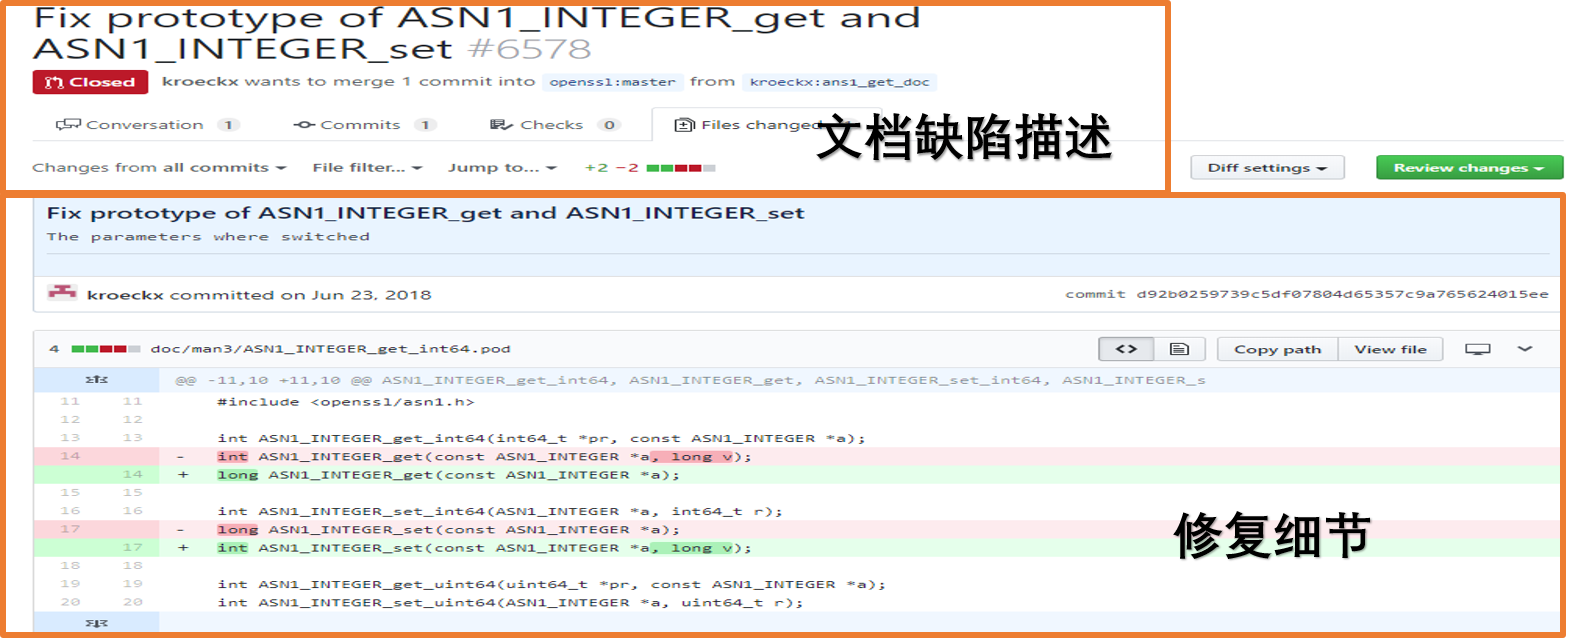
\includegraphics[width=0.8\linewidth]{figures/cp4-doc-bug.png}
	\caption{
		OpenSSL中接口用户手册缺陷修复记录。
	}
	\label{fig:4-4-doc-bug}
\end{figure}
\paragraph{现有文档}
虽然OpenSSL软件库提供了格式优良的自然语言描述的接口使用约束和解释,
然而在本文分析的15个应用软件中,依旧存在大量的接口误用缺陷。
对缺陷报告和文档进行分析后,现有的文档存在如下几个不足:
\begin{itemize}
	\item 文档自身存在错误。在OpenSSL的缺陷检测中,本文发现OpenSSL提供的官方文档中存在错误。
	在进行代码具体使用情况和文档描述后,作者提交了文档和接口缺陷报告(Issue-6569)。
	开发者在收到缺陷报告后,1天内对文档进行了修复,如图~\ref{fig:4-4-doc-bug}中所示。
	\item 文档利用率不足。一方面,软件库项目代码中本身存在接口误用。
	另一方面,客户端开发者则误用这些接口。
	在和开发者讨论原因时,超过一半的开发者表示,在遇到使用问题时更喜欢去Google或者Stack-overflow中搜索,
	而不是参考官方文档。
	\item 客户端未能感知软件库的更新。
	如图~\ref{fig:4-4-exim-bug}中所示,在exim项目中,作者在提交缺陷报告(ID-2316\footnote{https://bugs.exim.org/show\_bug.cgi?id=2316})后,开发者根据旧版本的用户手册认为缺陷不成立。
	然而,在OpenSSL最新的用户手册和最新的代码中,已经对相应的接口进行更新。
	在提交相应的说明后,开发者对缺陷修复。
\end{itemize}

总结来说,即使现有的软件库提供了格式良好的使用测试和参考用例,
开发者在遇到问题时,依旧首选网络平台进行咨询。
然而,根据调研~\cite{18-icse-stack}显示,网络平台中的代码质量并不可靠。
特别地,随时开源软件社区的蓬勃发展,大量的软件库缺少文档。
所以,现有的文档形式,难以满足用户的需求。
因此,本文基于缺陷模式,设计了面向C程序接口使用约束的领域特定语言IMSpec。
该语言旨在和现有的自然语言描述形成互补,以提供更好的描述接口使用约束。

\begin{figure}[b]
	\centering
	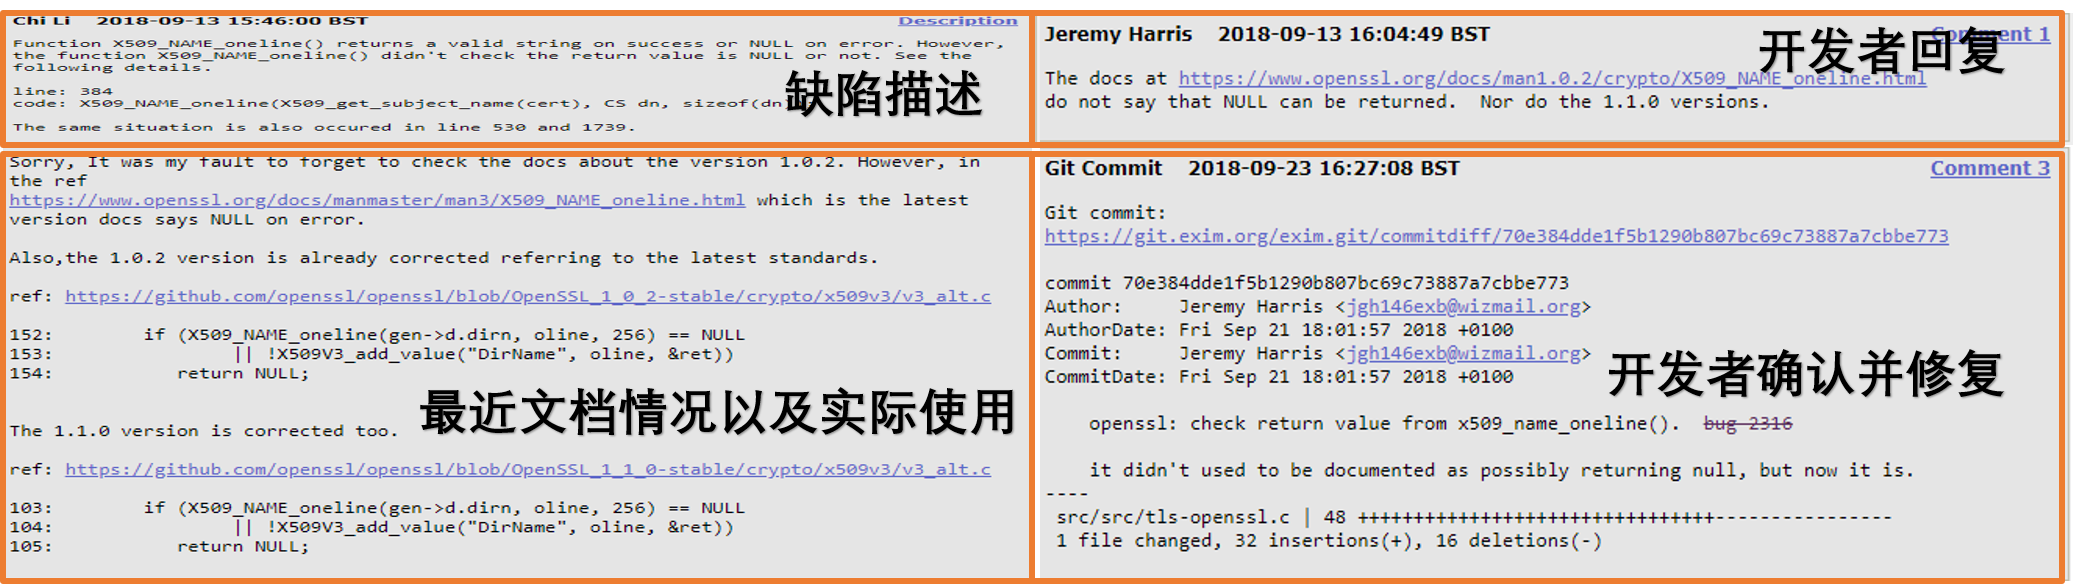
\includegraphics[width=\linewidth]{figures/cp4-exim-bug.png}
	\caption{
		exim项目中缺陷2316修复记录。
	}
	\label{fig:4-4-exim-bug}
\end{figure}

\paragraph{缺陷提交}
在缺陷检测后,本文作者针对于选择的缺陷细节进行深入分析,并提交缺陷报告给相应的开发者。
期初,在缺陷报告中只包含错误的位置和原因。
开发者很少反馈,或者希望作者提供更多的有效信息。
在此基础之上,作者丰富了缺陷报告,在报告中包含:缺陷位置、原因、具体路径信息和对比正确使用片段,
供开发者更好的理解缺陷。
面对改进后的缺陷报告,提交的多数报告被开发者接受与修复。
作者将缺陷报告提交中的经验总结如下:
\begin{itemize}
	\item 开发者更喜欢提交代码修复(Pull Request)。
	在缺陷提交的过程中,Linux内核的维护者表示只接受修复提交,
	Ubuntu的应用软件的开发者则更欢迎提交修复代码。
	相对的,OpenSSL开发者积极的在帮助作者进行缺陷修复。
	\item 提交策略。
	在缺陷报告提交初期,本文作者连续的提交数十个缺陷报告。
	获得回复较少,一个可能的原因为,开发者认为这样的缺陷报告是批量产生,质量不高。
	此后,作者降低提交频率。不仅获得了较多回复,同时缺陷的认可和修复率都提高。
	\item 缺陷报告信息要充分。
	如上文所述,丰富缺陷报告信息,能够有效的帮助开发者理解缺陷。
\end{itemize}

总结来说,缺陷提交需要大量的人力进行信息正确和确认。
在提交过程中,作者发现开发者更喜欢接收修复代码。
然而,缺陷修复需要大量的领域知识和上下文信息。
此外基于差异性的路径信息能够有效的帮助开发者理解缺陷原因,提供缺陷修复模式。
因此,在Tsmart-IMChecker工具集中,本文实现了基于差异性对比的缺陷结果展示工具IMDisplayer。

\begin{figure}[b]
	\centering
	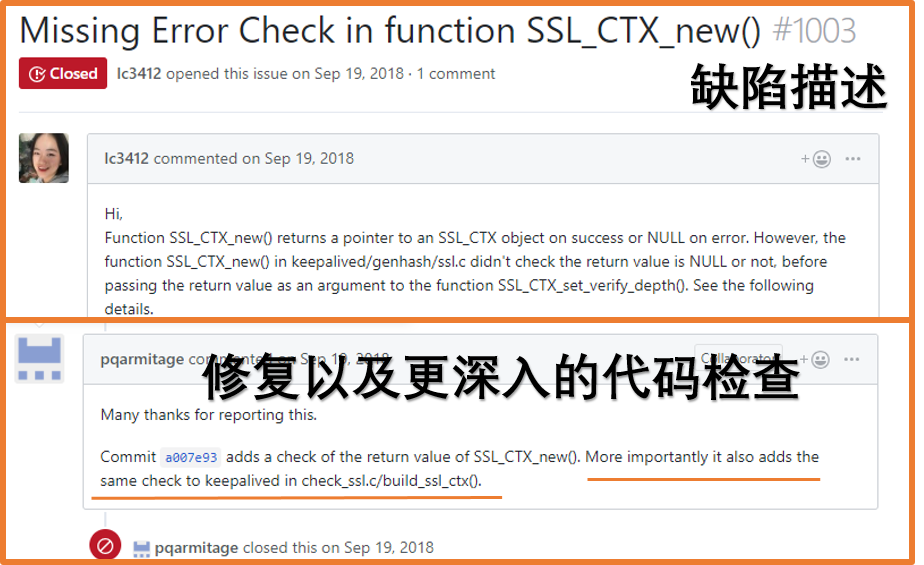
\includegraphics[width=0.8\linewidth]{figures/cp4-keepalived-fix.png}
	\caption{
		OpenSSL中接口用户手册缺陷修复记录。
	}
	\label{fig:4-4-keepalived-fix}
\end{figure}

\paragraph{开发者态度}
在缺陷报告的过程中,开发者展现了不同的态度。
一方面,开发对缺陷报告进行积极响应,例如OpenSSL的开发者多数在1天就就完成了缺陷的修复。
另一方面,开发者则更希望作者提供实际的运行轨迹或者提供修复代码,而不仅仅是缺陷报告。
特别地,本文将与开发者的交流和讨论中特殊发现总结如下,
\begin{itemize}
	\item 开发者自身忽视接口使用的约束。
	在实际开发过程中,开发者难以做到完全正确。
	即使是简单的参数检查和返回值检查,在大量的代码中,普遍存在这种缺陷。
	然而,这些缺陷难以通过人工的方式进行一一排查。
	特别地,当开发者认识到这些缺陷时,会对其他代码中同样的缺陷模式进行检测。
	如图~\ref{fig:4-4-keepalived-fix}所示,在keepalived项目中,在作者提交缺陷报告后,开发者不仅修复了对应的缺陷,还对其他的代码进行了类似缺陷的检测和修复。
	\item 特殊目的。
	虽然有些接口误用确实为缺陷,但是是开发者故意为之或者在特殊的应用内,无需修复。
	例如OpenSSL项目,提供了app/speed.c文件用于测试算法速度。
	因此在代码中,存在大量的缺少必要返回值检查的接口误用(IssueID-6575)。
	OpenSSL一个开发者认为这些误用在这个上下文中并不需要关注。
	然而,其他开发者认为这部分代码作为应用中的案例,是其他开发者的重要参考,需要重视。
	开发者进行了深入的讨论后,决定在后续的开发过程中进行统一处理(Assessed)。
	另一方面,由于C程序缺少异常处理机制,开发者会故意忽略部分异常检测。
	因为,软件设计时,本身就没有考虑这些情况。
\end{itemize}

总结来说,基于有效信息的缺陷报告能够获得开发者积极的反馈。
并不是所有的接口误用都会引起开发者的关注。
特别地,有一些误用是开发者故意为之。
例如,提高运行效率、C程序无法支持的异常处理情况和接口本身的特殊性等等。





\section{本章小结}
\label{sec:4.5}
本章将C程序接口使用约束描述语言IMSpec和规模化接口缺陷检测方法IMChecker在实际项目中进行应用。
为了帮助研究人员和开发者理解接口误用缺陷,本章整理了C程序接口缺陷数据集APIMU4C。
该数据集包含接口缺陷案例库以及接口缺陷测试集,以供检测工具的性能评估、针对性的工具选择和新的算法研究。
同时,本章设计并实现了可视化支撑的C程序接口缺陷检测工具集Tsmart-IMChecker,
并将工具集应用于开源项目缺陷检测中。
结果显示,Tsmart-IMChecker在Linux内核、OpenSSL库和Ubuntu系统应用软件的最新版本中,
共发现75个实际缺陷。其中62个已经被开发者确认,32个被开发者修复。